%
% Slides
% 
% Template by Sandrine Lefranc
%
%

\documentclass{beamer}
\usepackage[T1]{fontenc}
\usepackage[utf8]{inputenc} 

\usecolortheme{IAS2}
\usefonttheme{default}

\useinnertheme[shadow=true]{rounded}
\useoutertheme{infolines}

\setbeamerfont{block title}{size={}}
\setbeamercolor{titlelike}{parent=structure}

\definecolor{MyBackground}{rgb}{0.0, 0.0, 0.0}
\setbeamercolor{background canvas}{bg=MyBackground}

\setbeamercolor{normal text}{fg=white,bg=black}
\setbeamercolor{alerted text}{fg=red}
\setbeamercolor{example text}{fg=green!50!white}

\usepackage{amsmath}
\usepackage{verbatim}
\usepackage{array}
\usepackage{subfigure}
\usepackage{multirow}
\usepackage{colortbl}
\usepackage{slashbox}
\usepackage{verbatim}
\usepackage{multicol}
\usepackage{multimedia}
%\usepackage[]{algorithm2e} 
\usepackage{tikz}
\usetikzlibrary{arrows,shapes}
\newcommand{\omitme}[1]{}
\def\R{\mathbb{R}}
\DeclareMathOperator*{\argmin}{arg\,min}
\DeclareMathOperator*{\argmax}{arg\,max}

% hourglass
%\usepackage{fontawesome}
\newcommand{\faHourglass}{\faicon{hourglass}}

% smileys
\usepackage{wasysym}
\newcommand\good{{\color{green}\smiley}}
\newcommand\bad{{\color{red}\frownie}}

\newcommand{\checkmarkgreen}{{\textcolor{the_green} \checkmark}}
\newcommand{\Checkmark}{{\large{\checkmarkgreen}}}


\usepackage[loadonly]{enumitem}
\usepackage{url}
\usepackage{hyperref}


\newcommand{\commentaire}[1]{}
\newtheorem{prop}{Property}
\newtheorem{theo}{Theorem}
\newtheorem{books}{Reference books}
\newtheorem{code}{Source code for segmentation available from:}
\newtheorem{de}{Definition}
\newtheorem{cor}{Corollary}
\newcommand{\emdef}[1]{\alert{#1}}
\newtheorem{Encadre}[theorem]{}
 
\newcolumntype{C}{>{\centering\arraybackslash$}m{2cm}<{$}}
\newcolumntype{H}{@{}>{\rule{0pt}{8mm}}m{0pt}@{}}

\definecolor{the_green}{rgb}{0.075,0.375,0.375}
\definecolor{darkgreen}{rgb}{0.1,0.5,0}
\definecolor{darkred}{rgb}{0.8,0,0}
\definecolor{newpurple}{rgb}{0.8,0.35,0.8}
\definecolor{newturquoise}{rgb}{0.2,0.8,0.82}
\newcommand \important[1]{\textcolor{darkred}{#1}}
\newcommand \medium[1]{\textcolor{blue}{#1}}
\usepackage{multimedia}

\definecolor{darkorange}{rgb}{0.8,0.5,0.2}
\definecolor{lightgray}{rgb}{0.97,0.97,0.97}
\definecolor{lightorange}{rgb}{0.9,0.66,0.04}
\definecolor{lightgreen}{rgb}{0.48,0.8,0.48}
\definecolor{newwhite}{rgb}{1,1,1}
\definecolor{newred}{rgb}{1,0,0}
\definecolor{newblue}{rgb}{0,0,1}

\definecolor{newlightblue}{rgb}{0.55,0.4,1}



\newcommand \myblue[1]{\textcolor{newblue}{#1}}
\newcommand \mywhite[1]{\textcolor{newwhite}{#1}}
\newcommand \mylightblue[1]{\textcolor{newlightblue}{#1}}
\newcommand \mypurple[1]{\textcolor{newpurple}{#1}}
\newcommand \myturquoise[1]{\textcolor{newturquoise}{#1}}
\beamerboxesdeclarecolorscheme{green}{lightgreen}{lightgray}
\beamerboxesdeclarecolorscheme{blue}{newlightblue}{lightgray}
\beamerboxesdeclarecolorscheme{orange}{lightorange}{lightgray}
\beamerboxesdeclarecolorscheme{equation}{white}{lightgray}
\newcommand \colorref[1]{\textcolor{mygreen}{#1}}
\newcommand{\relief}{\only{\color{blue}}}

\definecolor{myyellow2}{rgb}{0.933,0.909,0.666}%PaleGoldenrod 238 232 170 blue
 \definecolor{myyellow}{rgb}{1,1,0.878}%LightYellow 255 255 224 yellow
 \definecolor{myblue}{rgb}{0.9,0.9,1} %Khaki	240 230 140 yellow2
 \definecolor{myred}{rgb}{1,0.8,0.725} %PeachPuff 255 218 185 red
 \definecolor{redless}{rgb}{1,0.6,0.5} %PeachPuff 255 218 185 red
 \definecolor{mygreen}{rgb}{1,0.898,0.719}
\definecolor{myorange}{rgb}{1,0.933,0.840}
\definecolor{pink}{rgb}{1,0,0.35}

%%--- subfigure weirdness
\renewcommand{\thesubfigure}{\thefigure.\arabic{subfigure}} \makeatletter
\renewcommand{\p@subfigure}{}
\renewcommand{\@thesubfigure}{\thesubfigure:\hskip\subfiglabelskip} \makeatother

%%--- subfigure sizes
\newcommand\scale{0.7} 

%%--- math symbols
\newcommand{\esp}{\mathbb{E}}
\newcommand{\bM}{\mathbb{M}}
\newcommand{\dist}{\mathrm{dist}}
\newcommand{\cond}{\mathrm{cond}}
\newcommand{\integ}{\mathcal{I}}
\newcommand{\entropy}{\mathcal{H}}
\newcommand{\seg}{\mathcal{S}}
\newcommand{\cM}{\mathcal{M}}
\newcommand{\comp}{\mathcal{C_N}}
\newcommand{\ntwk}{\mathcal{N}}
\newcommand{\myciting}[1]{{\footnotesize{\tt{\textcolor{magenta}{[#1]}}}}}
\newcommand{\myred}[1]{{\textbf{#1}}}

% Custom colors
\usepackage{color}
\definecolor{deepblue}{rgb}{0,0,0.5}
\definecolor{deepred}{rgb}{0.6,0,0}
\definecolor{deepgreen}{rgb}{0,0.5,0}

%%--- notes
%\setbeameroption{show notes}

%%--- beginning of the talk -----

\title{Sammba-MRI: SmAll MaMmals BrAin MRI in Python}
\author[Salma Bougacha]{Salma Bougacha, Nachiket Nadkarni, Cl\'ement Garin, Marc Dhenain}%{Salma Bougacha}
\date{2018, June 22}
\titlegraphic{%
   
\includegraphics[scale=.4]{Images/mircen_black_bg.png}\hspace*{3cm}~%
   
\includegraphics[scale=.4]{Images/cyceron_black_bg.png}\hspace*{0.5cm}%
}
\usenavigationsymbolstemplate{}
\institute[APPNING]{APPNING Workshop, Paris}

\usepackage{lmodern}

%\usepackage{biblatex}
%\addbibresource{biblio.bib}
\usepackage{caption}
\captionsetup[figure]{labelformat=empty}% redefines the caption setup of the figures environment in the beamer class.

\usepackage{fancybox}
\usepackage{mathtools}

\setbeamertemplate{footline}{
\leavevmode%
\hbox{\hspace*{-0.06cm}
\begin{beamercolorbox}[wd=.2\paperwidth,ht=2.25ex,dp=1ex,center]{author in head/foot}%
	\usebeamerfont{author in head/foot}\insertshortauthor%~~(\insertshortinstitute)
\end{beamercolorbox}%
\begin{beamercolorbox}[wd=.6\paperwidth,ht=2.25ex,dp=1ex,center]{section in head/foot}%
	\usebeamerfont{section in head/foot}\insertshorttitle
\end{beamercolorbox}%
\begin{beamercolorbox}[wd=.2\paperwidth,ht=2.25ex,dp=1ex,right]{section in head/foot}%
	\usebeamerfont{section in head/foot}\hspace*{2em}
	\insertframenumber{} / \inserttotalframenumber \hspace*{2ex}
\end{beamercolorbox}}%
\vskip0pt%
}


\newenvironment{colorblock}[2]
{
\begin{beamerboxesrounded}[upper=#1,lower=#2,shadow=true]}
{\end{beamerboxesrounded}}

\begin{document}

\frame{
\titlepage
}
%-TOC with current section and all associated subsections highlighted-------
\AtBeginSection[] % Do nothing for \section*
{\begin{frame}<beamer> 
\frametitle{Outline}
\tableofcontents[currentsection] 
\end{frame}}
%-TOC with current section and current subsection highleited---------
\AtBeginSubsection[] % Do nothing for \subsection*
{ \begin{frame}<beamer> \frametitle{Outline} \tableofcontents[current,currentsubsection] \end{frame} }
%\begin{python}
%class MyClass(Yourclass):
%    def __init__(self, my, yours):
%        bla = '5 1 2 3 4'
%        print bla
%\end{python}


%---------------------------------------------------------
\begin{frame}{Frame title 1}
\frametitle{Features}

  \begin{center} 
    \begin{columns}

      \begin{column}{0.5\textwidth}
 \begin{itemize}
 \item Bruker DICOM to NIFTI conversion
 \vspace*{0.1\linewidth}
 \item Registration to standard
 \vspace*{0.1\linewidth}
 \item Between modalities registration 
 %\myciting{Buckner et al., 2009, Crossley et al., 2014}
 \end{itemize}
      \end{column}

      \begin{column}{0.5\textwidth}
 \begin{itemize}
 \item Template creation
 \vspace*{0.2\linewidth}
 \item Perfusion FAIR processing
 \end{itemize}
      \end{column}

     \end{columns}
   \end{center}


\end{frame}
%---------------------------------------------------------
\begin{frame}{Frame title 1}
\frametitle{Results}
  \begin{center} 
    \begin{columns}
	\hspace*{1cm}

      \begin{column}{0.45\textwidth}

        \begin{tabular}{c} 
	   \includegraphics[width=0.6\linewidth]{Images/atlas_overlays_dim-1pt6.png}\\
		{High registration accuracy}
        \end{tabular}   
        \hspace*{.4cm}
        \begin{tabular}{c} 
	   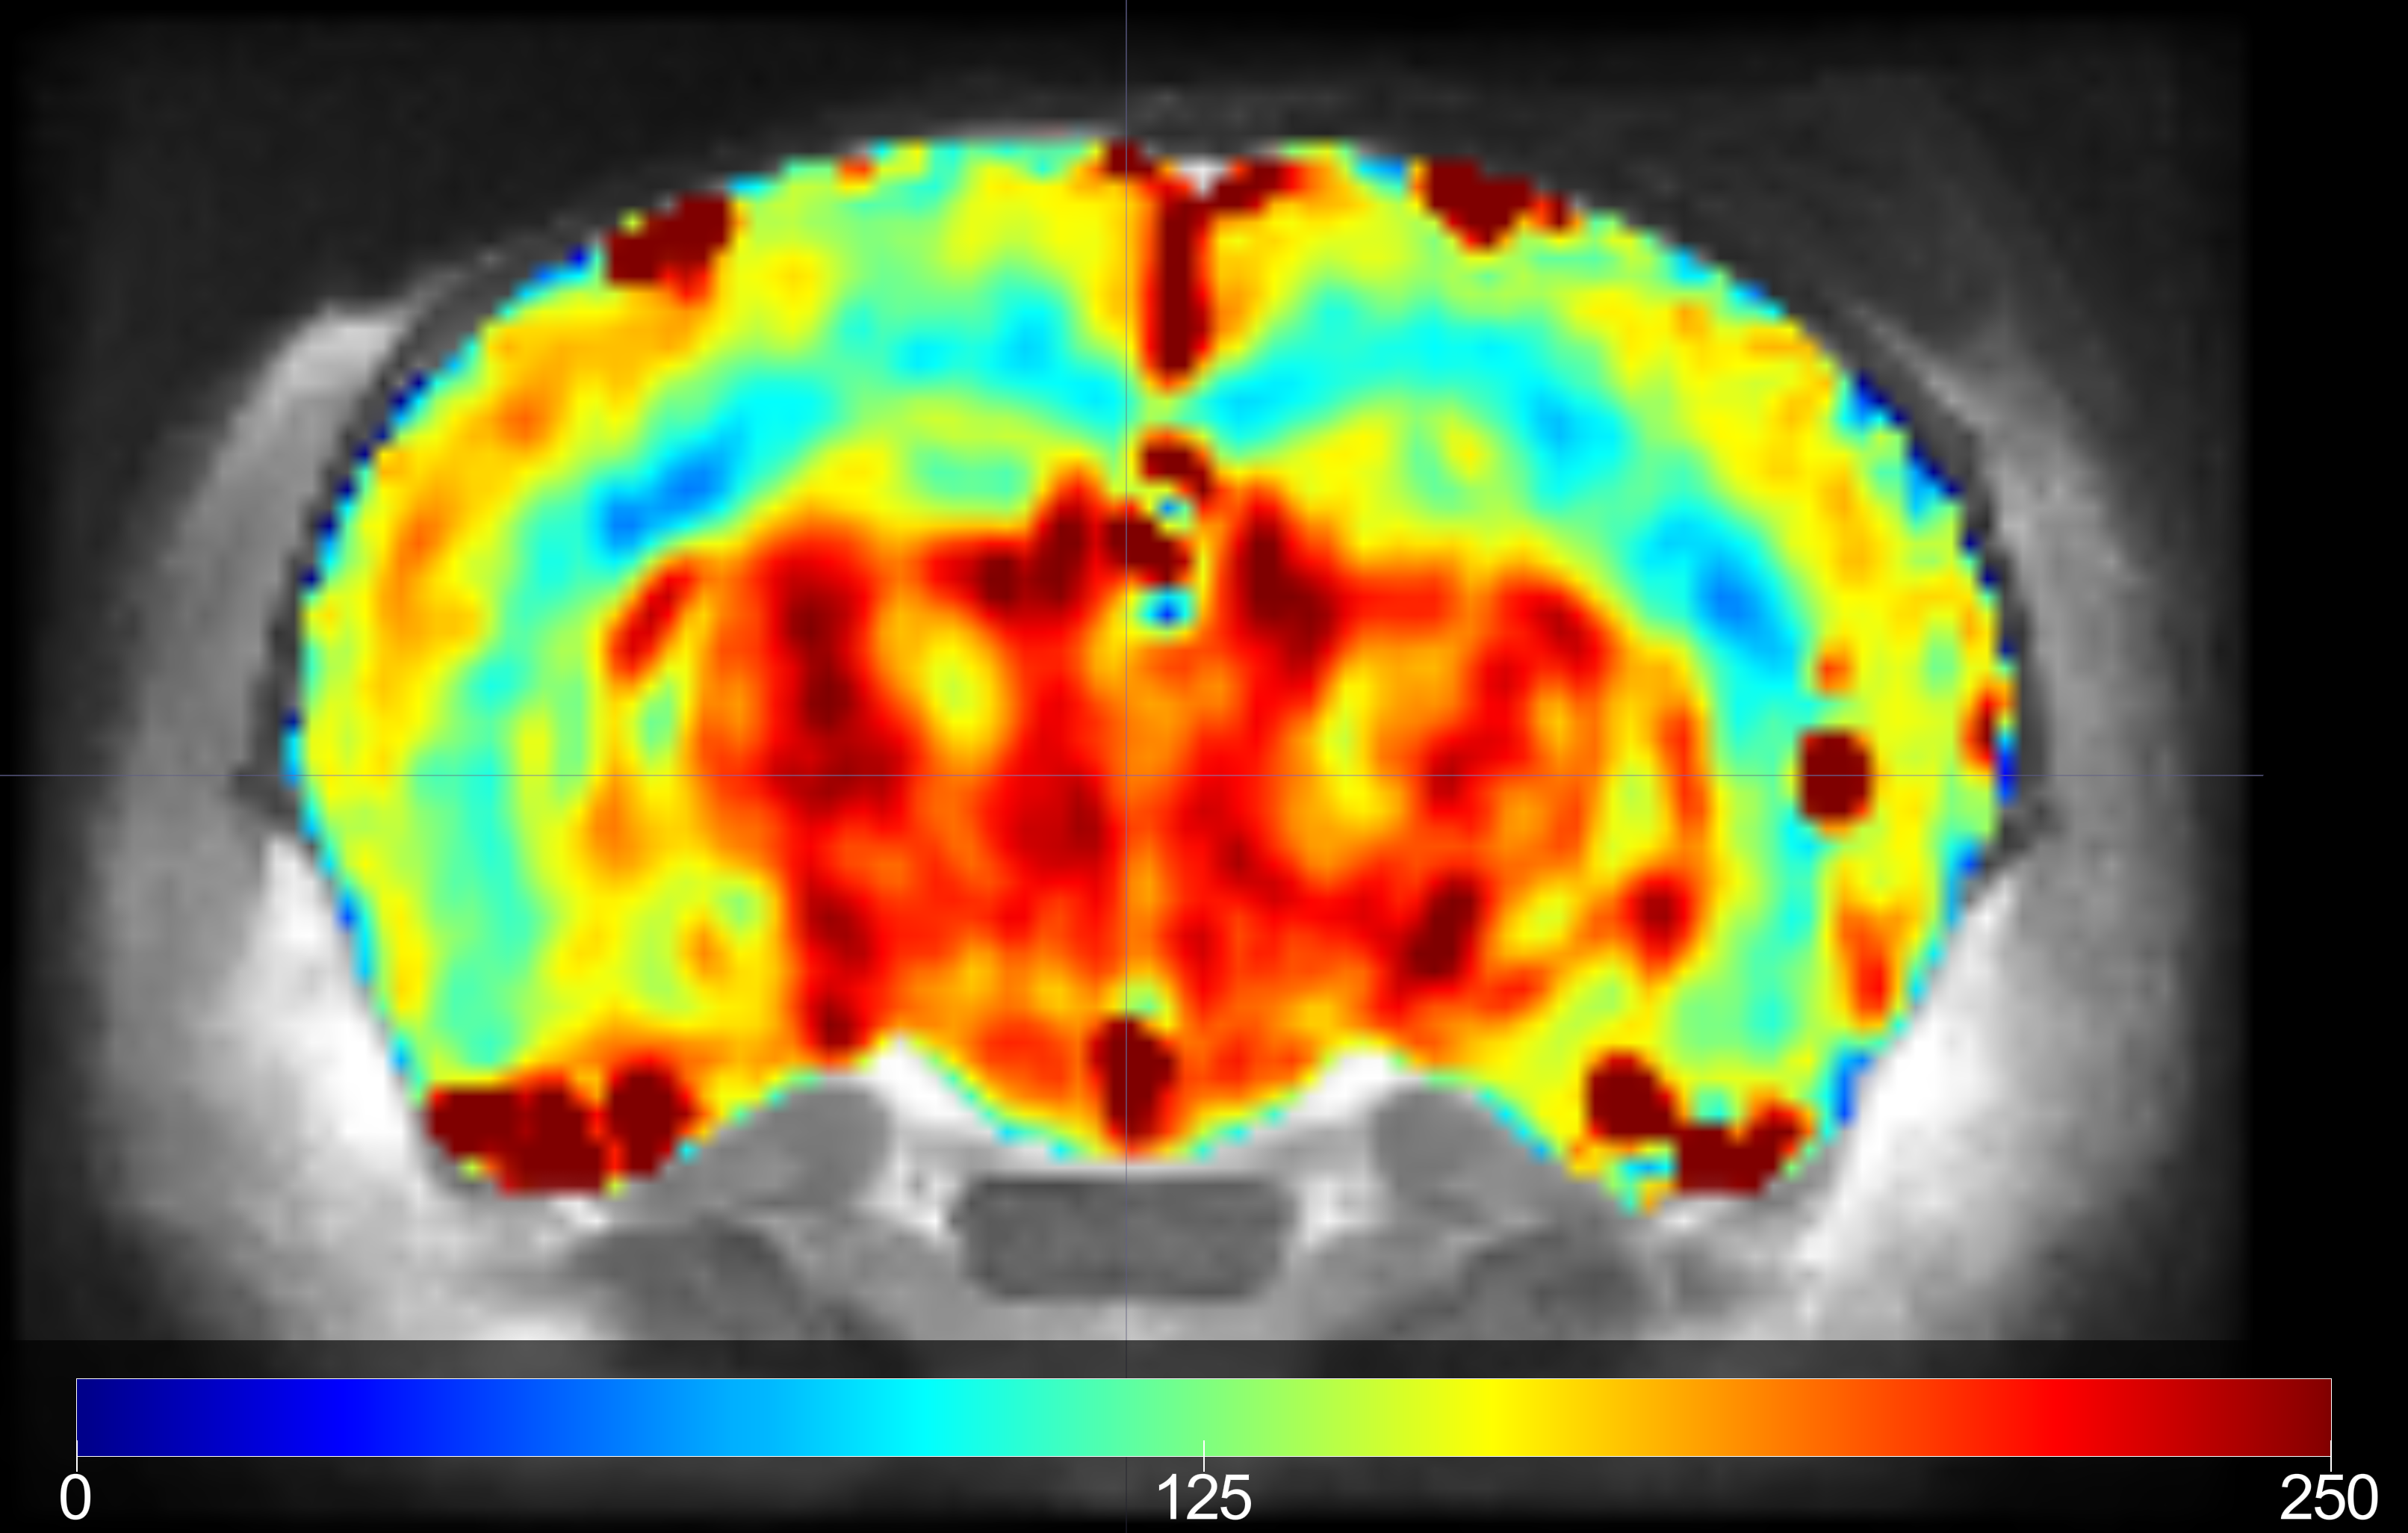
\includegraphics[width=0.6\linewidth]{Images/mean_cbf_mricron2.png}\\
		{Cerebral blood flow}\\
		{quantification}
        \end{tabular}   
      \end{column}

      \begin{column}{0.55\textwidth}
        \begin{tabular}{c} 
	   \includegraphics[width=0.7\linewidth]{Images/component26_not_annotated.png}\\
		{Straightforward resting state}\\
		{networks extraction}
        \end{tabular}   
       \begin{tabular}{c} 
		\includegraphics[width=.7\linewidth]{Images/sfn_template.jpg}\\
		{Fine mouse lemur template}\\
		\end{tabular}   
       \end{column}

     \end{columns}
   \end{center}

\end{frame}
%---------------------------------------------------------
\begin{frame}{Frame title 1}
\frametitle{You want to try it ?}
\vspace*{3cm}
\begin{center}
\huge{\textcolor{yellow}{\url{https://sammba-mri.github.io}}}
\end{center}
\vspace*{4cm}
%\includegraphics[width=.4\linewidth]{Images/python_logo.png}
%\hspace*{4cm}
%\includegraphics[width=.2\linewidth]{Images/github_logo_name3.png}
\end{frame}
%---------------------------------------------------------
%
%\section*{Bibliography}
%{\tiny
%\bibliographystyle{plain}
%\bibliography{biblio}
%}
\end{document}

